\documentclass{article}

\usepackage{amsmath,graphicx,parskip,mathrsfs,subfigure}
\usepackage{fancyhdr}
\usepackage{amsthm,amssymb}
\usepackage{setspace}
\usepackage{epstopdf}
\usepackage[left=3cm,right=3cm,top=3cm,bottom=3cm]{geometry}

\pagestyle{fancy}
\lhead{Samuel Huberman}
\chead{MSE1022:HW2}
\rhead{999157923}

\begin{document}
\section*{Part A}
\subsection*{a}
\begin{align*}
 F&=-\frac{dV}{dr}\\
  &=-\frac{d}{dr}(-Ar^{-n}+Br^{-m})\\
  &=-Anr^{-n-1}+Bmr^{-m-1}\\
\end{align*}
At equilibrium $r_0$, $F=0$:
\begin{align*}
 0&=-Anr^{-n-1}+Bmr^{-m-1}\\
 r_0 &=\left(\frac{Bm}{An}\right)^{\frac{1}{m-n}}
\end{align*}
\subsection*{b}
At $r_0$, the potential energy:
\begin{align*}
 V(r_0) &=\frac{-A}{\left(\frac{Bm}{An}\right)^{\frac{n}{m-n}}}+\frac{B}{\left(\frac{Bm}{An}\right)^{\frac{m}{m-n}}}
\end{align*}
For LJ, $A=4\epsilon \sigma ^6$ and $B=4\epsilon \sigma ^{12}$:
\begin{align*}
 r_0 &=\left(\frac{\sigma ^{6}m}{n}\right)^{\frac{1}{m-n}}\\
 V(r_0) &=\frac{-4\epsilon \sigma ^6}{\left(\frac{\sigma ^{6}m}{n}\right)^{\frac{n}{m-n}}}+\frac{4\epsilon \sigma ^{12}}{\left(\frac{\sigma ^{6}m}{n}\right)^{\frac{m}{m-n}}}
\end{align*}

\begin{figure}[h!]
\centering
\subfigure[]{
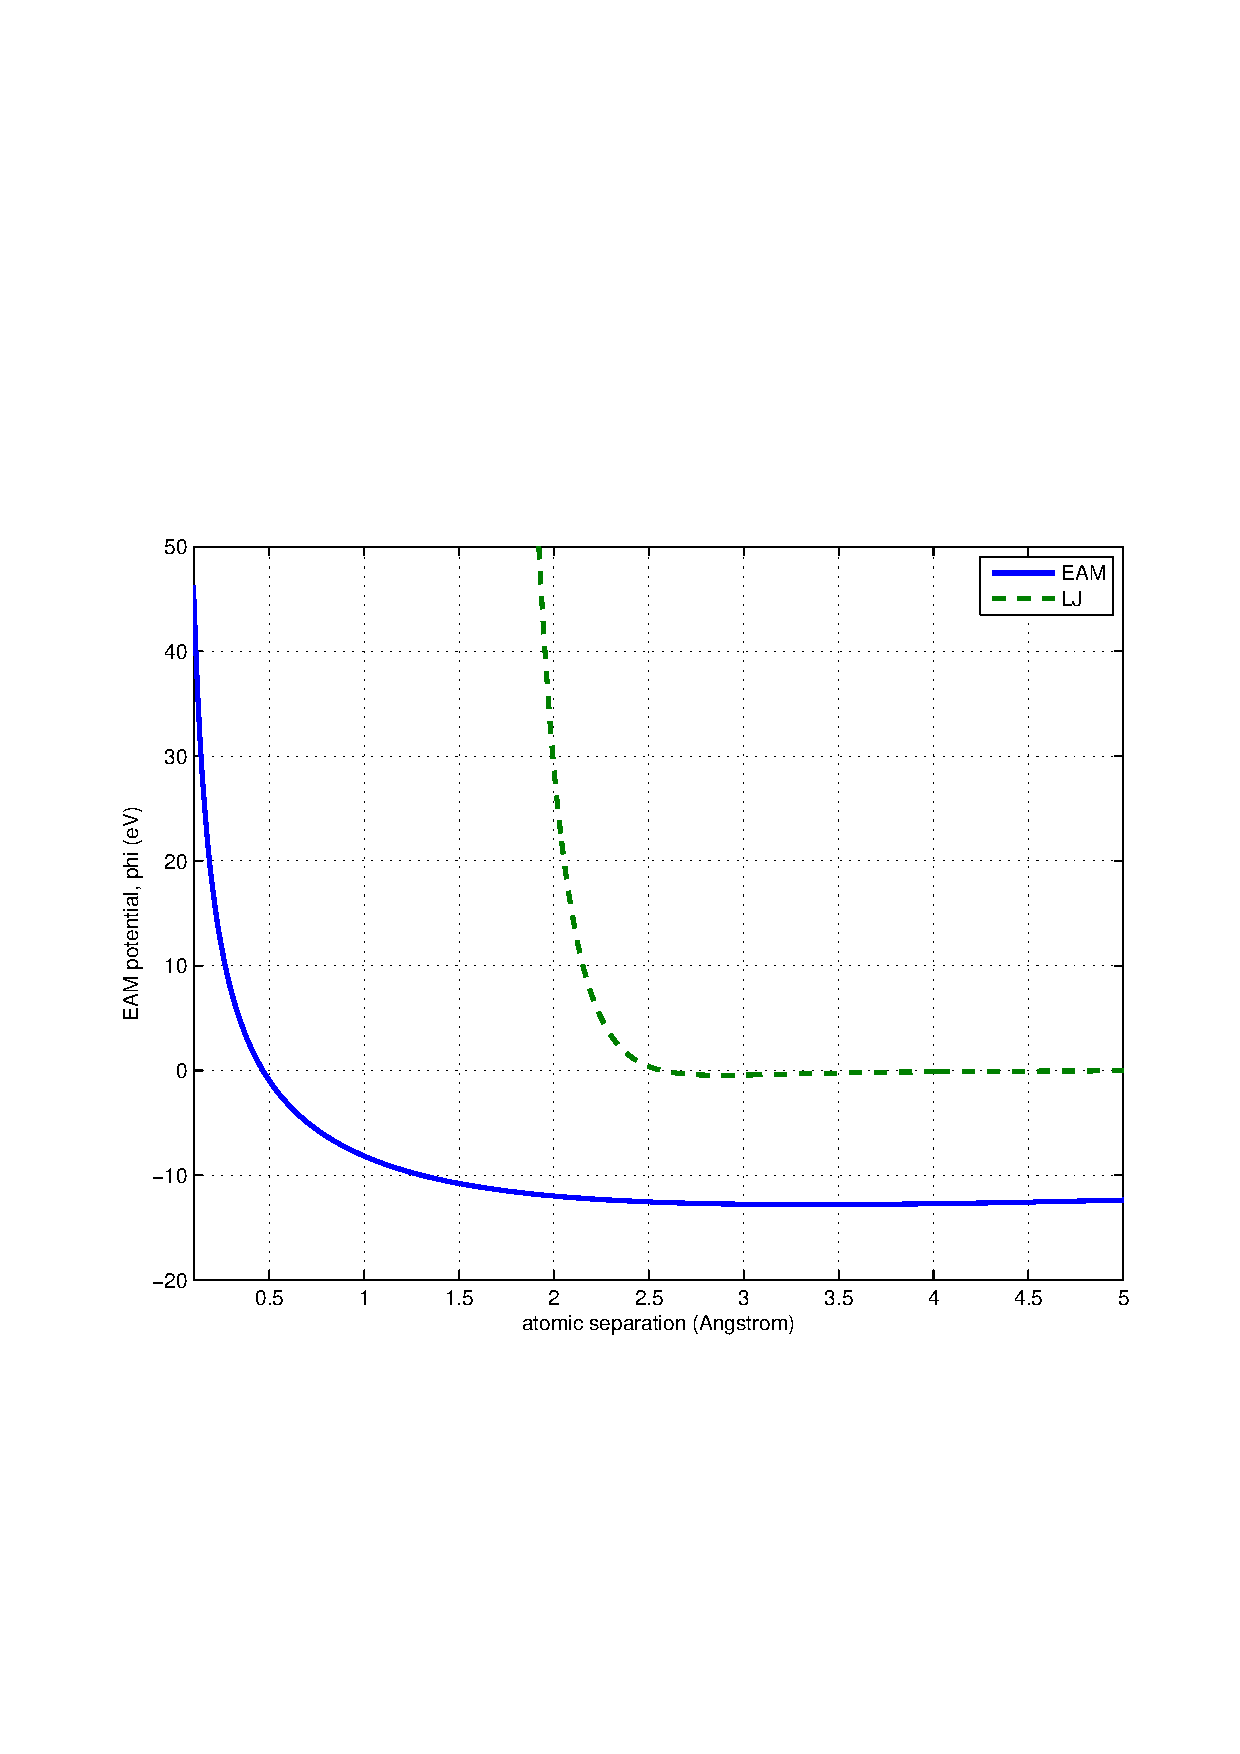
\includegraphics[totalheight=0.25\textheight]{fig2}
%\caption{Plot of LJ potential}
\label{fig:aNicePicture}
}
\subfigure[]{
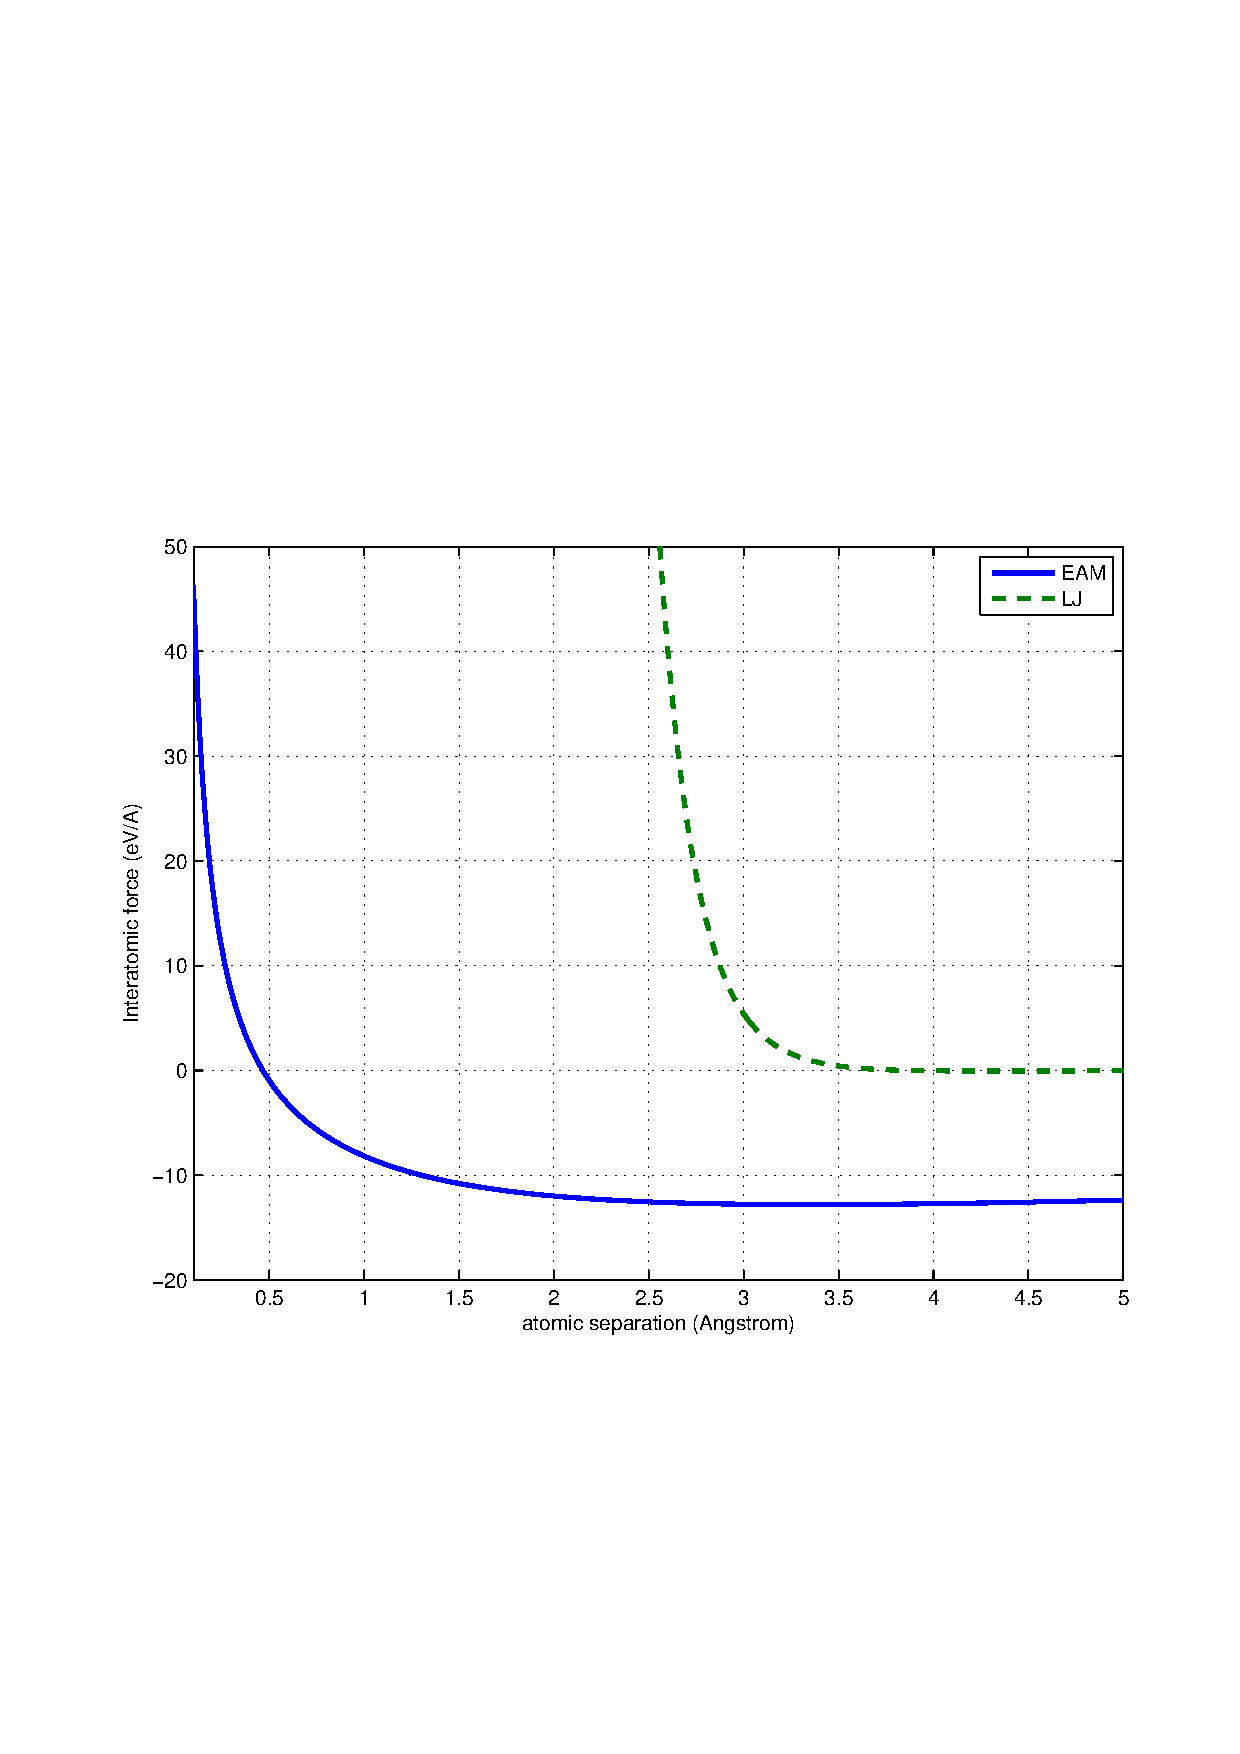
\includegraphics[totalheight=0.25\textheight]{fig3}
%\caption{Plot of LJ potential}
\label{fig:aNicePicture}
}
\caption{(a) Potential Energy (b) Force}
\end{figure}
\subsection*{c}
For MgO $A=4A_0e^2$,$B=B$ and NaCl $A=A_0e^2$,$B=B$: 
\begin{align*}
 \frac{r_{0MgO}}{r_{0NaCl}} &=\frac{9B}{4A_0e^2}^{\frac{1}{8}}/\frac{9B}{A_0e^2}^{\frac{1}{8}}\\
	&=\frac{1}{4}
\end{align*}
According to experiments, MgO has a lattice constant of about 4.18 Ang while NaCl has a lattice constant of 5.65 Ang. This indicates that this form of potential is not suitable for one or both of these compounds.
%\newpage
\section*{Part B}

\subsection*{Code}
\subsubsection*{a}
\begin{verbatim}
function genvel()
  global kboltz mvsq2e sys
  t=sqrt(3*sys.contemp*kboltz/mvsq2e/sys.mass)
  for i = 1 : 1 : sys.natoms
     sys.vx(i) = (-1.+2.*rand())*t;
     sys.vy(i) = (-1.+2.*rand())*t;
     sys.vz(i) = (-1.+2.*rand())*t;
  end
  if sum(sys.vx(:))+sum(sys.vy(:))+sum(sys.vz(:))>1E-10
    genvel();
  end
\end{verbatim}
\subsubsection*{b}
\begin{verbatim}
function verlet()
  global mvsq2e sys
  dtmf = sys.dt^2 / mvsq2e / (sys.mass);
  for i = 1 : 1 : sys.natoms
     sys.rx(i) =2*sys.rxk1(i)-sys.rxk(i) + (dtmf) * sys.fx(i);
     sys.ry(i) =2*sys.ryk1(i)-sys.ryk(i) + (dtmf) * sys.fy(i);
     sys.rz(i) =2*sys.rzk1(i)-sys.rzk(i) + (dtmf) * sys.fz(i);     
     sys.vx(i) = (sys.rxk1(i)-sys.rxk(i))/(sys.dt);
     sys.vy(i) = (sys.ryk1(i)-sys.ryk(i))/(sys.dt);
     sys.vz(i) = (sys.rzk1(i)-sys.rzk(i))/(sys.dt);
  end
  force();
\end{verbatim}
\subsubsection*{c}
\begin{verbatim}
function velrescale()
 global kboltz mvsq2e sys
  ekin();
  for i = 1 : 1 : sys.natoms
     sys.vx(i) = sqrt(sys.contemp/sys.temp)*sys.vx(i);
     sys.vy(i) = sqrt(sys.contemp/sys.temp)*sys.vy(i);
     sys.vz(i) = sqrt(sys.contemp/sys.temp)*sys.vz(i);
  end
\end{verbatim}
\subsubsection*{d}
\begin{verbatim}
function steep()
  global kboltz mvsq2e sys
  eta=0.01;
     while max(abs(sys.fx(:))) > sys.precision
     	sys.rx(:) = sys.rx(:)+eta*sys.fx(:);
        force();
     end
     while max(abs(sys.fy(:))) > sys.precision
     	sys.ry(:) = sys.ry(:)+eta*sys.fy(:);
        force();
     end
     while max(abs(sys.fz(:))) > sys.precision
     	sys.rz(:) = sys.rz(:)+eta*sys.fz(:);
        force();
     end
function conjgrad(conjg,cg,equil)
  global kboltz mvsq2e sys
  eta=0.00001;
      tic        
        sys.h(:,:) =sys.fk(:,:)+sum(sys.fk(:,:).*sys.fk(:,:),1)...
                    /sum(sys.fk1(:,:).*sys.fk1(:,:),1)*sys.h(:,:);
        sys.r(:,:) = sys.r(:,:)+eta*sys.h(:,:);
        sys.rx(:)=sys.r(:,1);
        sys.ry(:)=sys.r(:,2);
        sys.rz(:)=sys.r(:,3);
        sys.fk1(:,:)=[sys.fx(:),sys.fy(:),sys.fz(:)];
        force();
        sys.fk(:,:)=[sys.fx(:),sys.fy(:),sys.fz(:)];
        sys.l=sys.l+1;
        fprintf(conjg, '% 8d % 20.8f\n', sys.l, ...
                abs(max(norm(sys.fk))-max(norm(sys.fk1))));	
        figure(1);
        data=load('conjgrad_108.dat');
        plot(data(:,1),data(:,2));
    toc
\end{verbatim}
\subsubsection*{e}
\begin{figure}[h!]
\centering
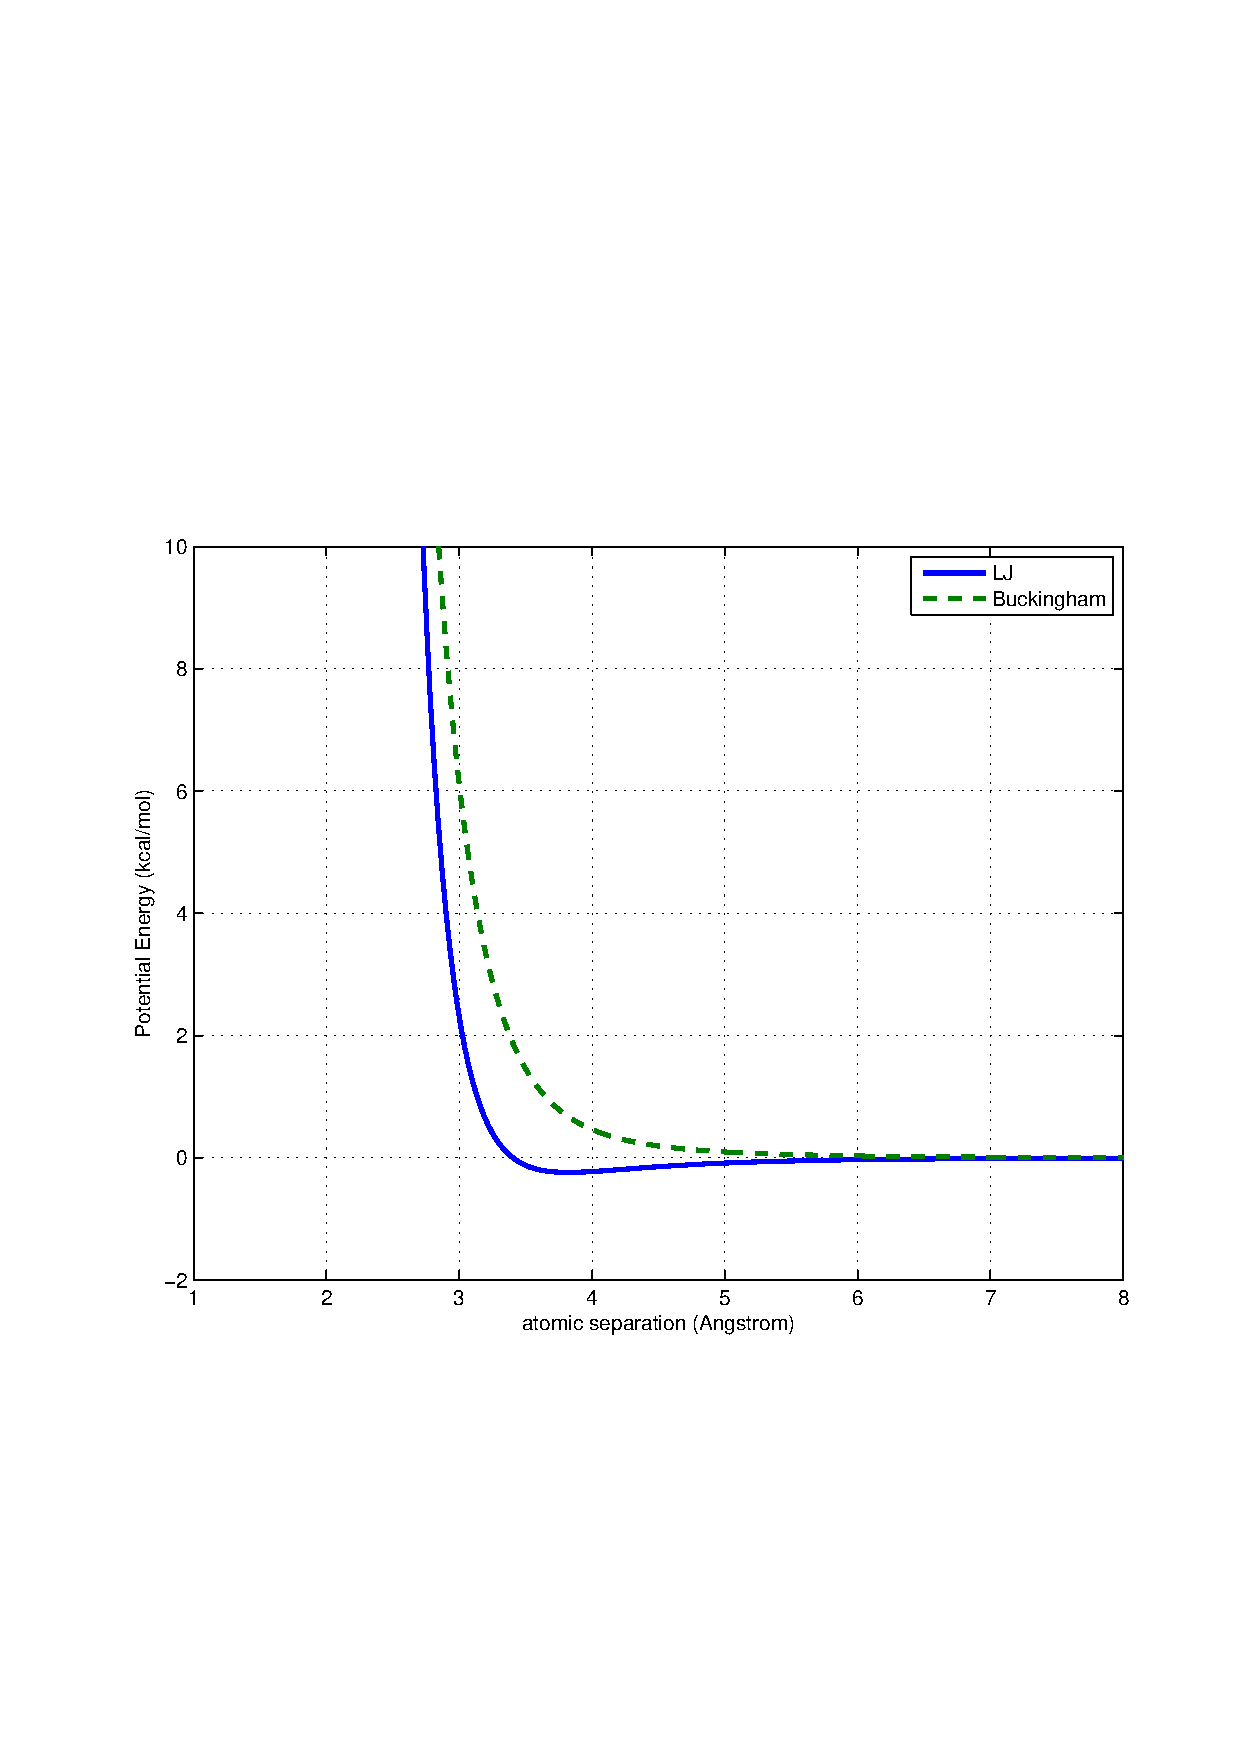
\includegraphics[totalheight=0.4\textheight]{fit}
\caption{Fitting of Buckingham potential to LJ Potential}
\label{fig:aNicePicture}
\end{figure}
\begin{verbatim}
function buck()
...
 %fit parameters:
 a=1.69e-8*6.241509*10^11*23.06055;
 b=1/0.273*6.241509*10^11*23.06055;
 c=102e-12*6.241509*10^11*23.06055;
...
 ffac = (-b*a*exp(-b*sqrt(rsq)))+6*c*sqrt(rsq)^(-7);
 sys.epot = sys.epot + a*exp(-b*sqrt(rsq))-c/sqrt(rsq)^(-6);
\end{verbatim}
\subsection*{Discussion}

From Figure 3, the randomly generated velocities results in a system temperature closer to the target temperature of 300K than the velocities from the restart file.
From Figure 4, the behaviour of the basic Verlet and velocity Verlet schemes are similar in terms of temperature, kinetic and potential energy for the simple system. However, the total energy fluctuates about some value for the basic Verlet scheme, but remains remarkably constant for the velocity Verlet scheme (as desired for NVE).
From Figure 5, velocity scaling correctly brings the system to the desired temperature.
From Figure 6, the steepest descent algorithm converges while the conjugate gradient algorithm does not. Perhaps, this is because the conjugate gradient algorithm cannot find the global minimum, but instead falls into a local minimum and in trying to move out of the this minimum, moves atoms too close to one another and consequently diverges.
From Figures 7 and 8, the Buckingham potential appears to produce similar temperatures and kinetic energies to the Lennard-Jones potential. However, the potential energy does not match (differ by 12 orders of magnitude). This is likely the result of the poor fit parameters.
Note: Argon has a melting temperature of around 87K and thus the simulations at 200K and 300K are either in the liquid or gas phase.


%\newpage
\subsection*{Results}
\begin{figure}[h!]
\centering
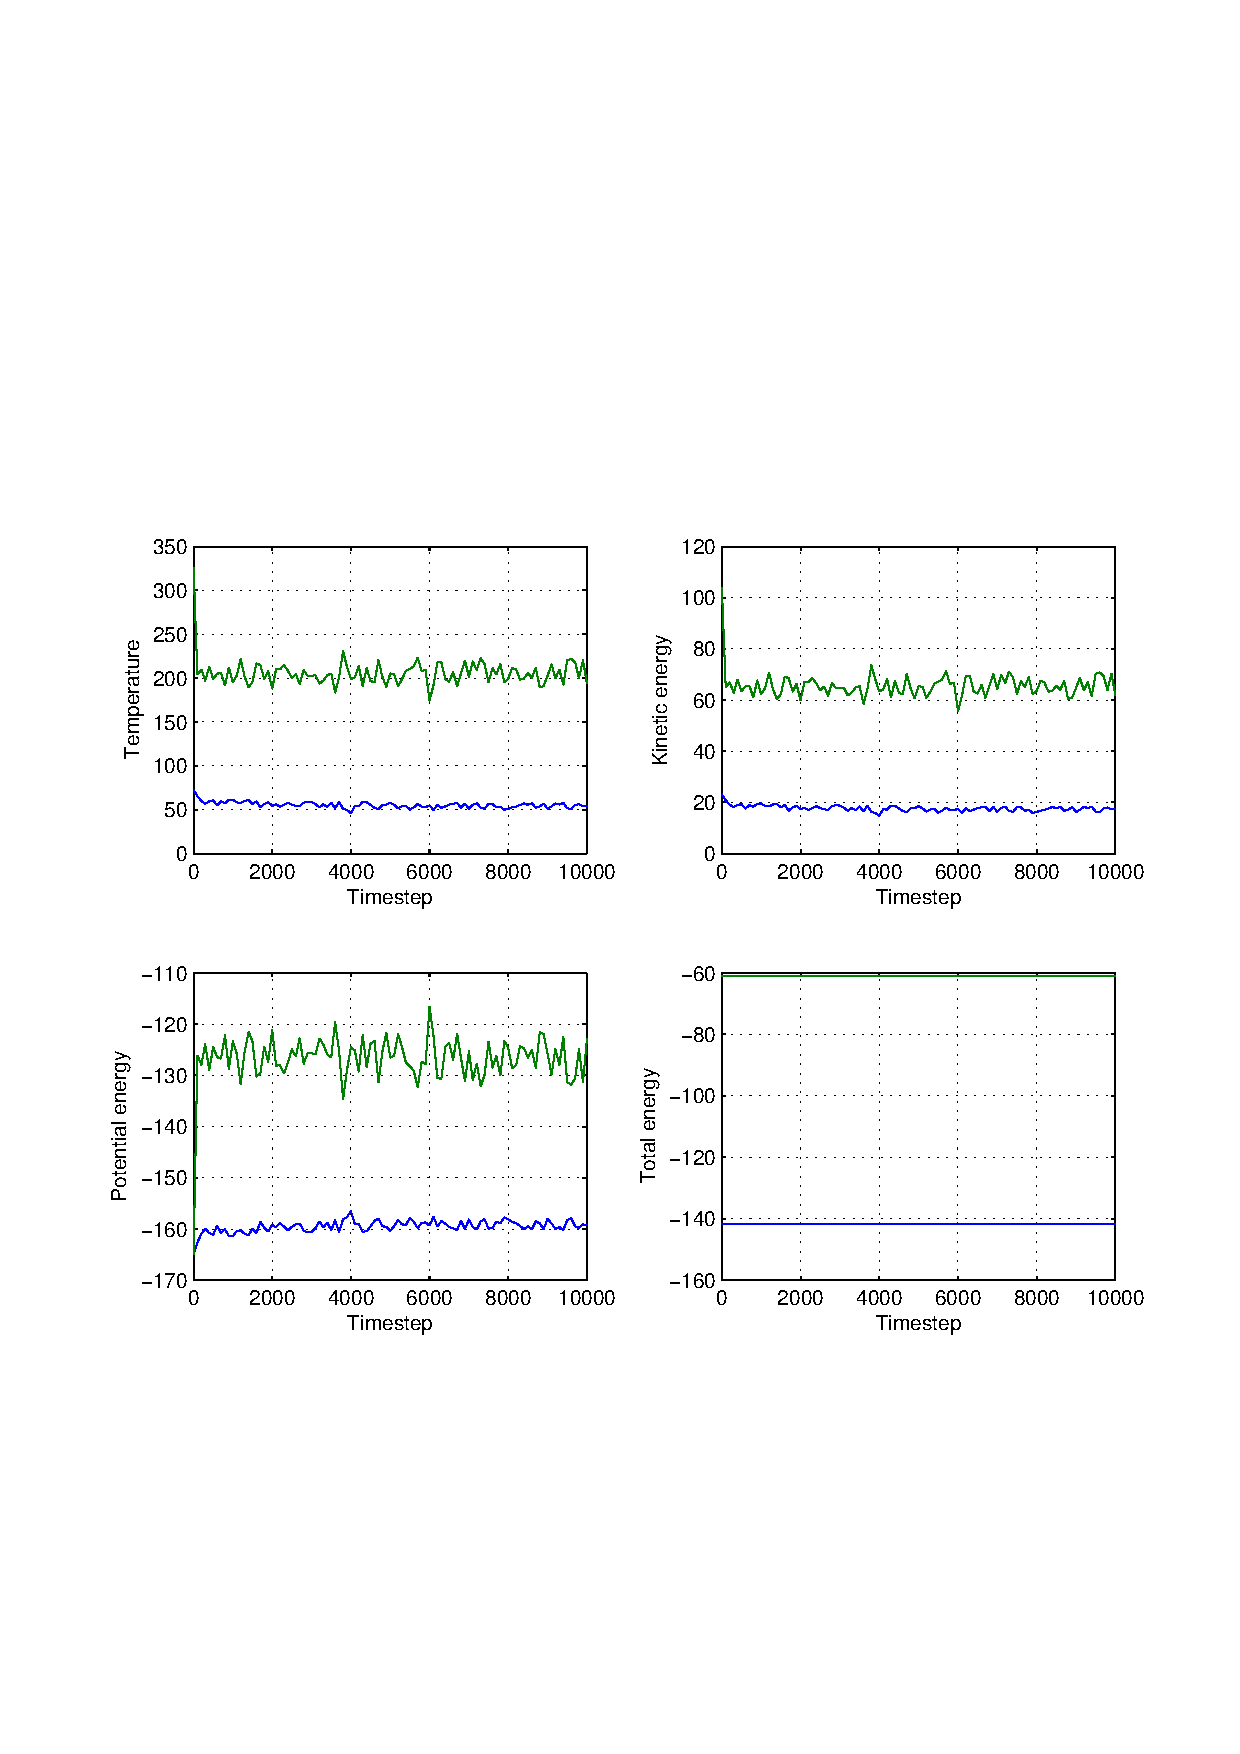
\includegraphics[totalheight=0.4\textheight]{partba}
\caption{Comparision between input velocities (Blue) and randomly generated velocities (Green)}
\label{fig:aNicePicture}
\end{figure}
\begin{figure}[h!]}
\centering
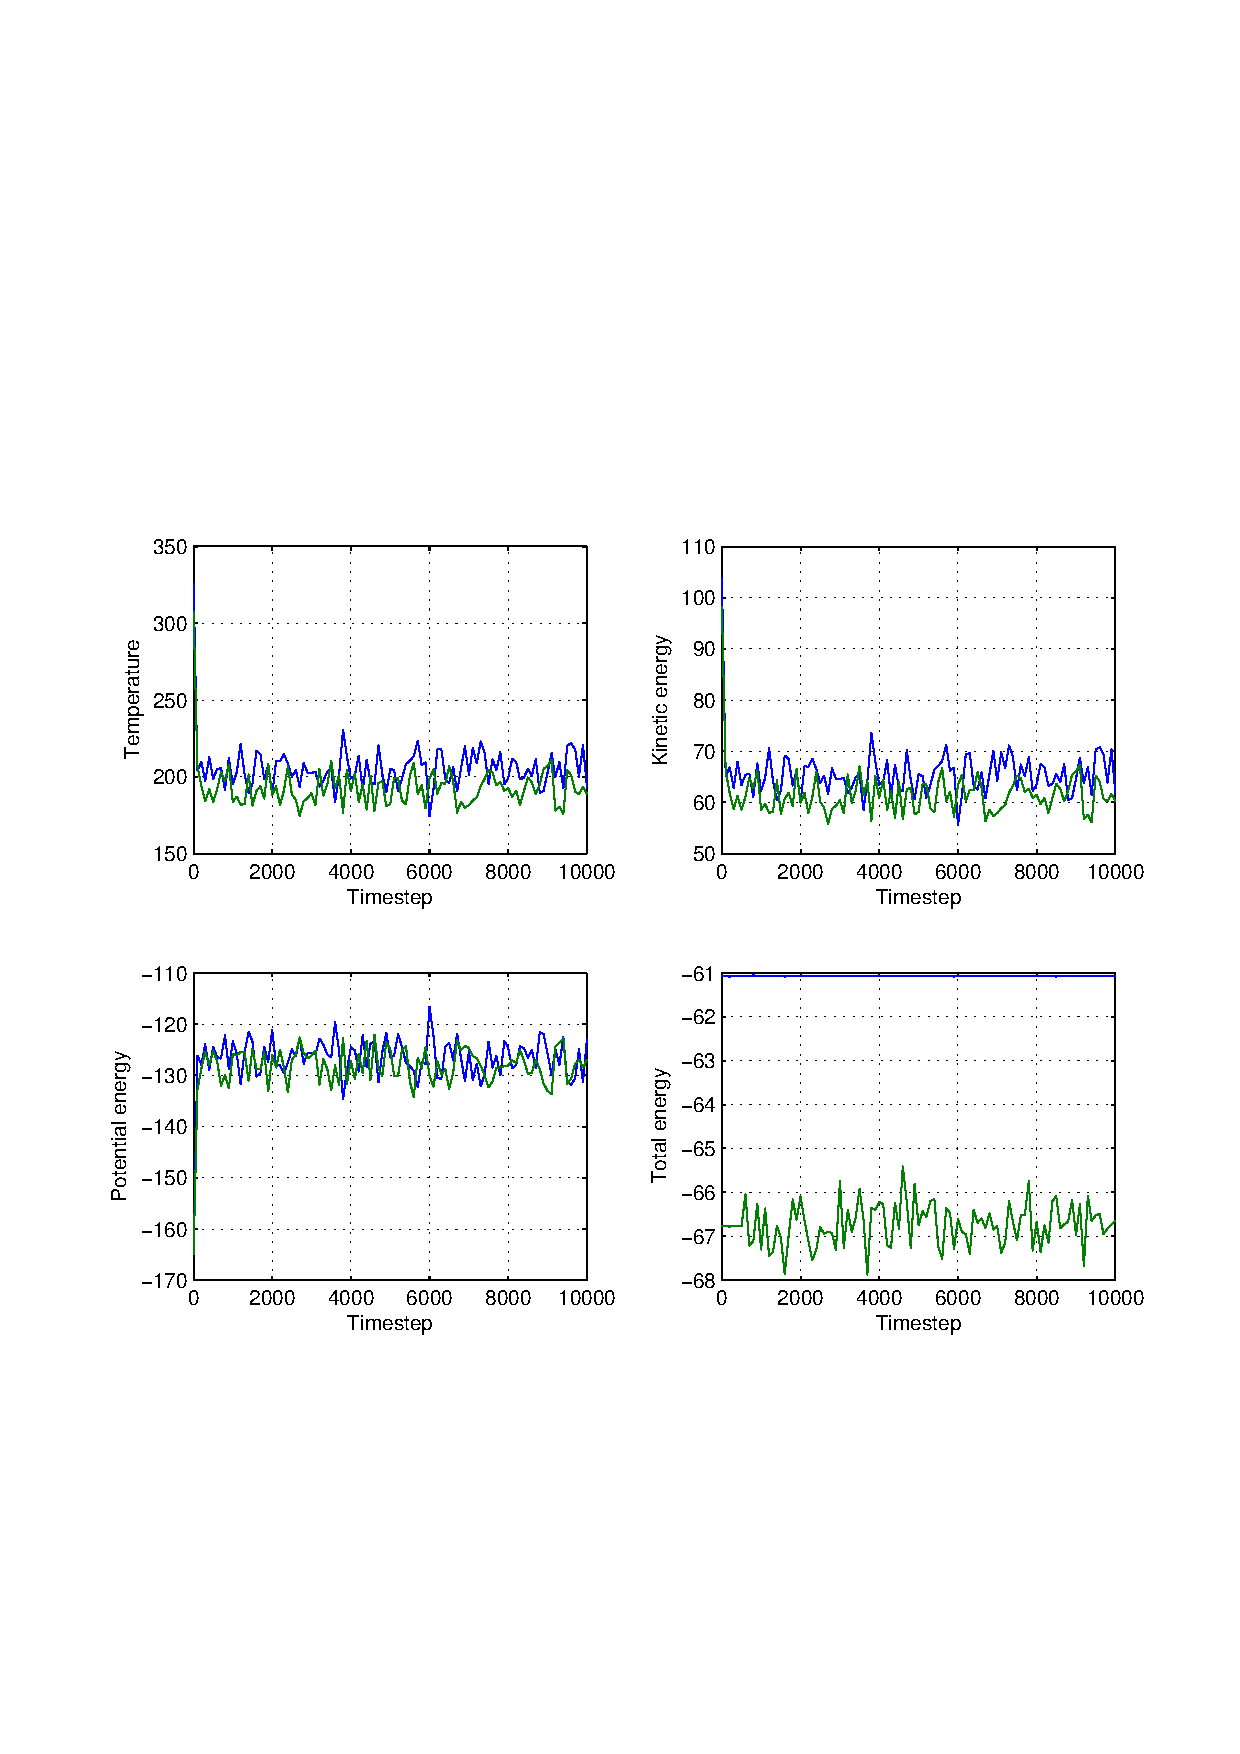
\includegraphics[totalheight=0.4\textheight]{partbb}
\caption{Comparision between Velocity Verlet (Blue) and Basic Verlet (Green)}
\label{fig:aNicePicture}
\end{figure}
\begin{figure}[!h]
\centering
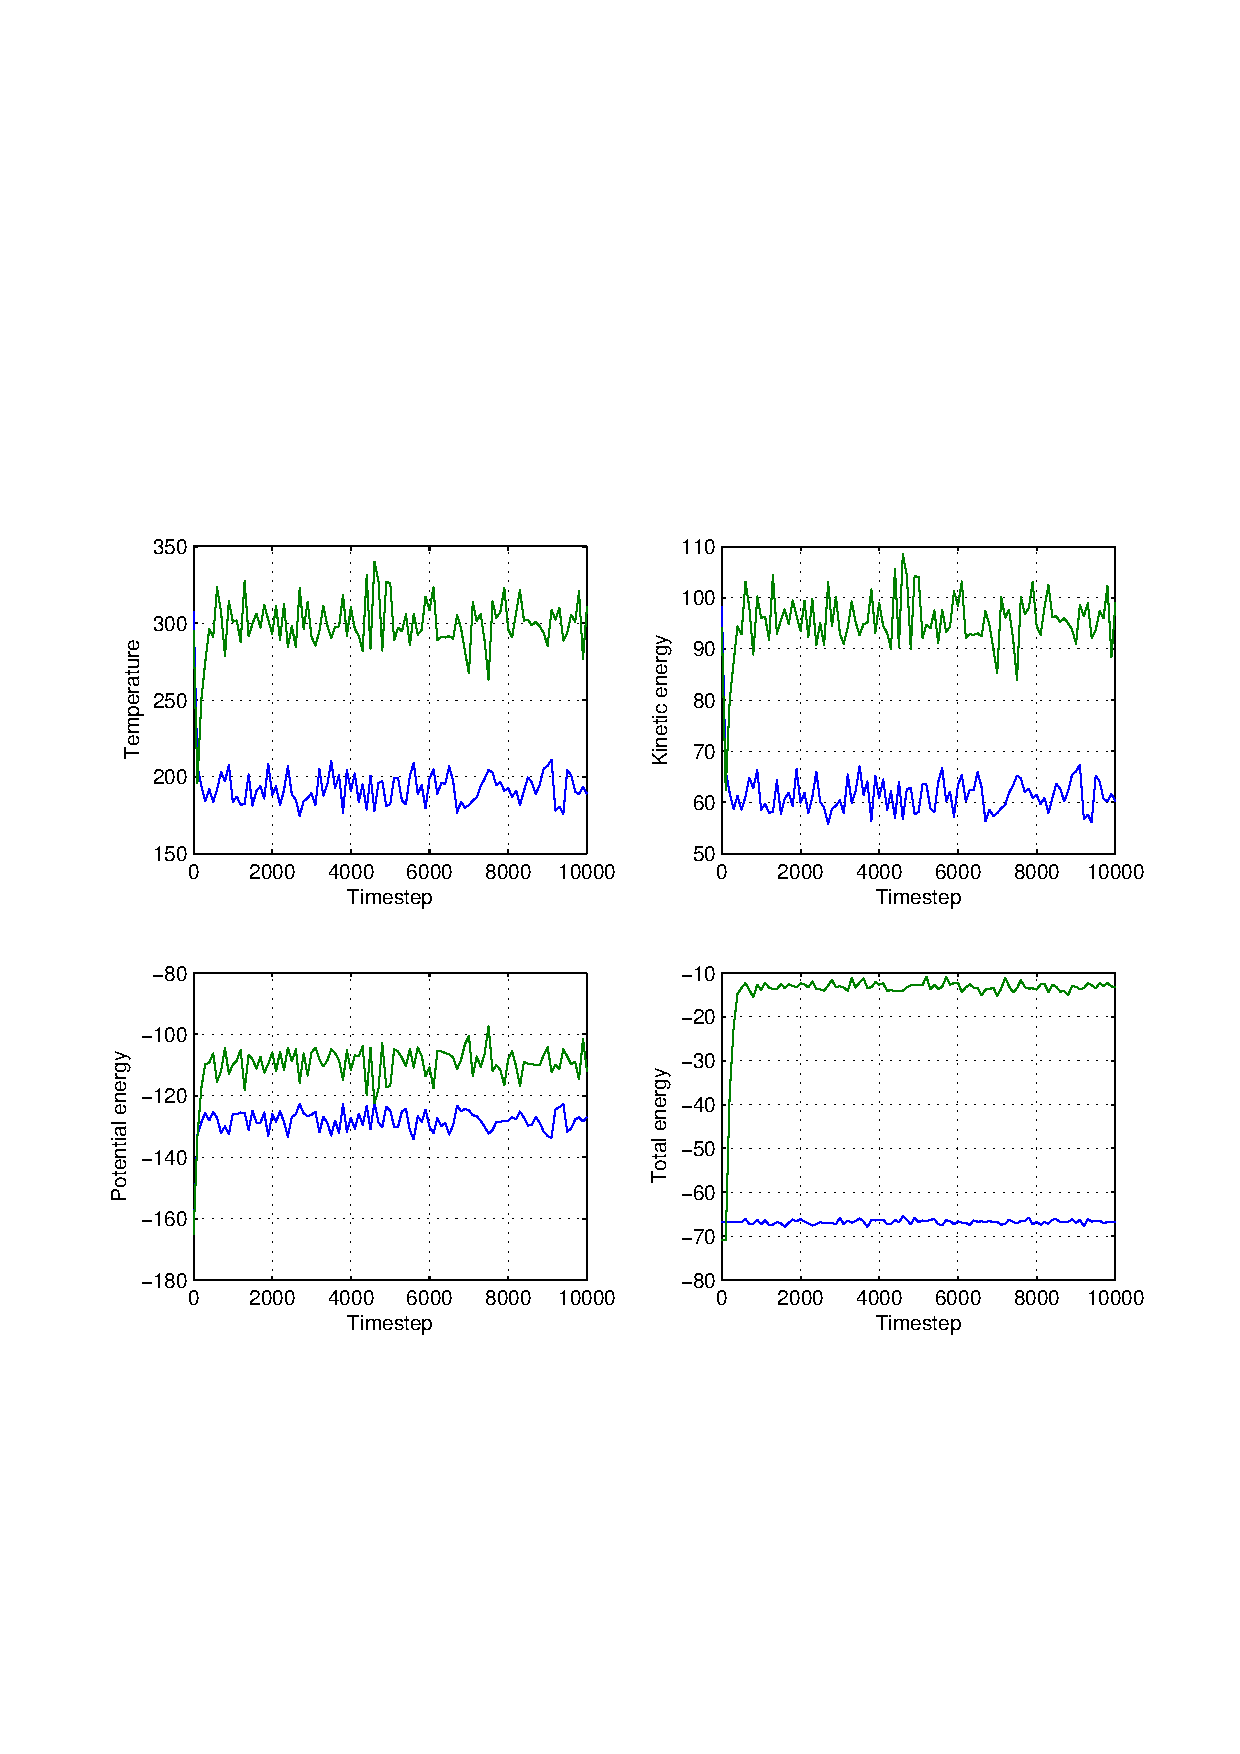
\includegraphics[totalheight=0.4\textheight]{partbc}
\caption{Comparision between Basic Verlet (Blue) and Basic Verlet with velocity scaling (Green) }
\label{fig:aNicePicture}
\end{figure}
\begin{figure}[!h]
\centering
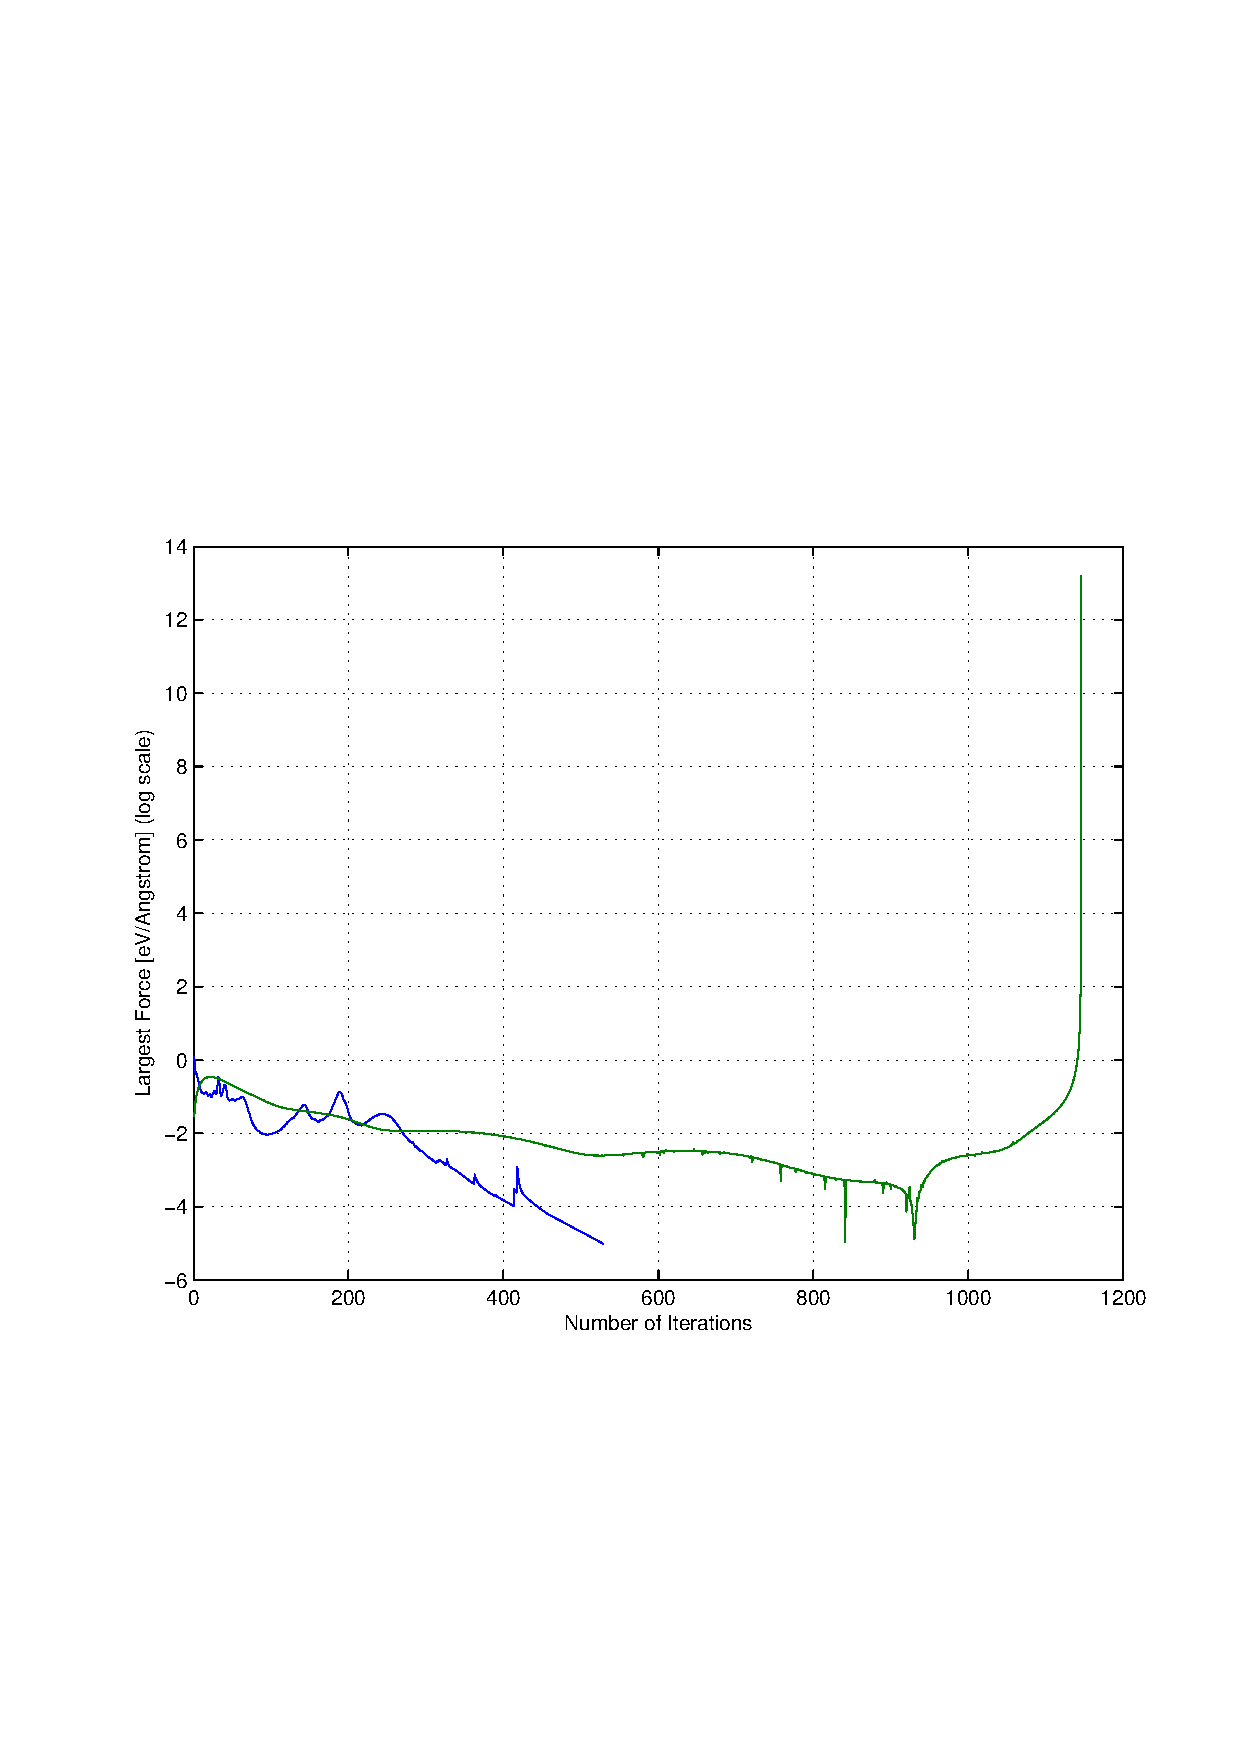
\includegraphics[totalheight=0.4\textheight]{partbd}
\caption{Comparision between Steepest Gradient (Blue) and Conjugate Gradient (Green)}
\label{fig:aNicePicture}
\end{figure}
\begin{figure}[!h]
\centering
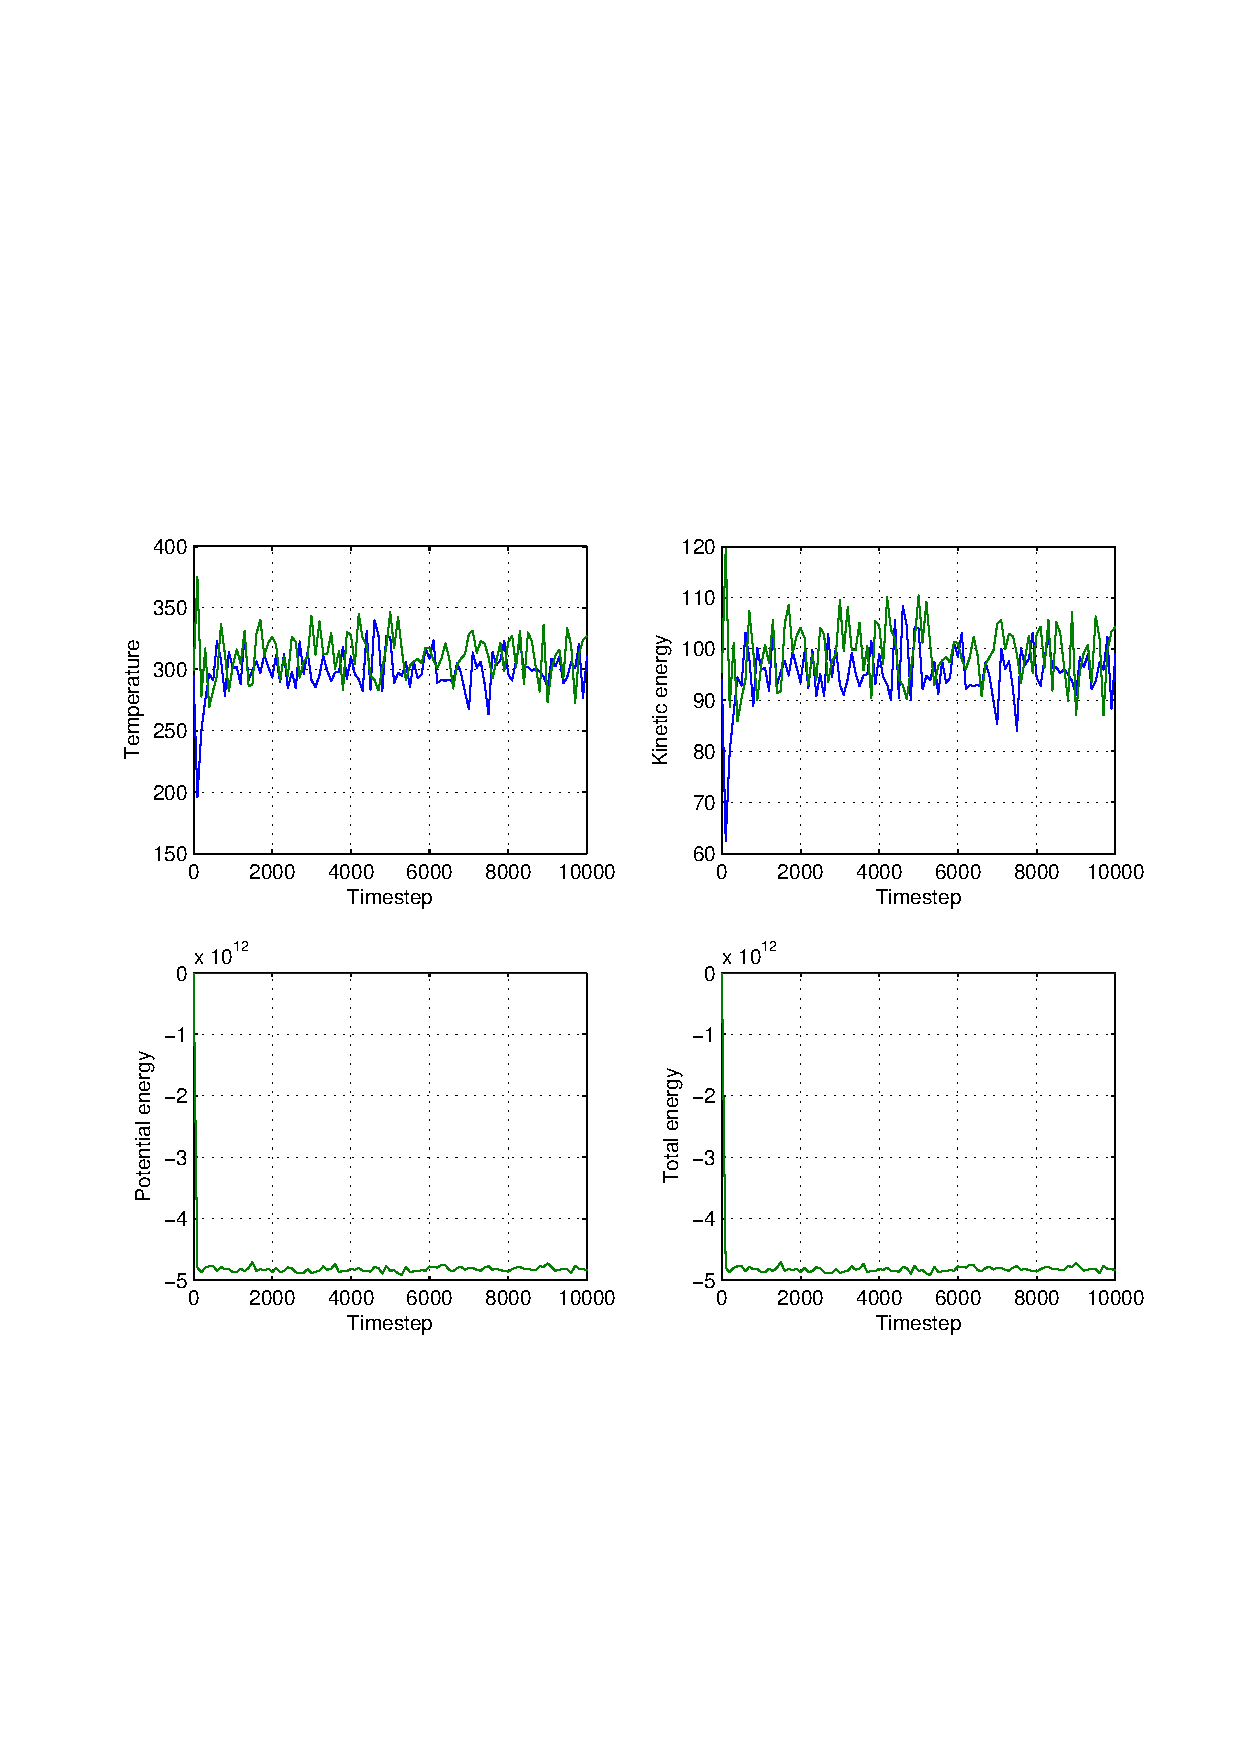
\includegraphics[totalheight=0.4\textheight]{partbe}
\caption{Comparision between LJ potential (Blue) and Buckingham Potential (Green)}
\label{fig:aNicePicture}}
\end{figure}
\begin{figure}[!h]
\centering
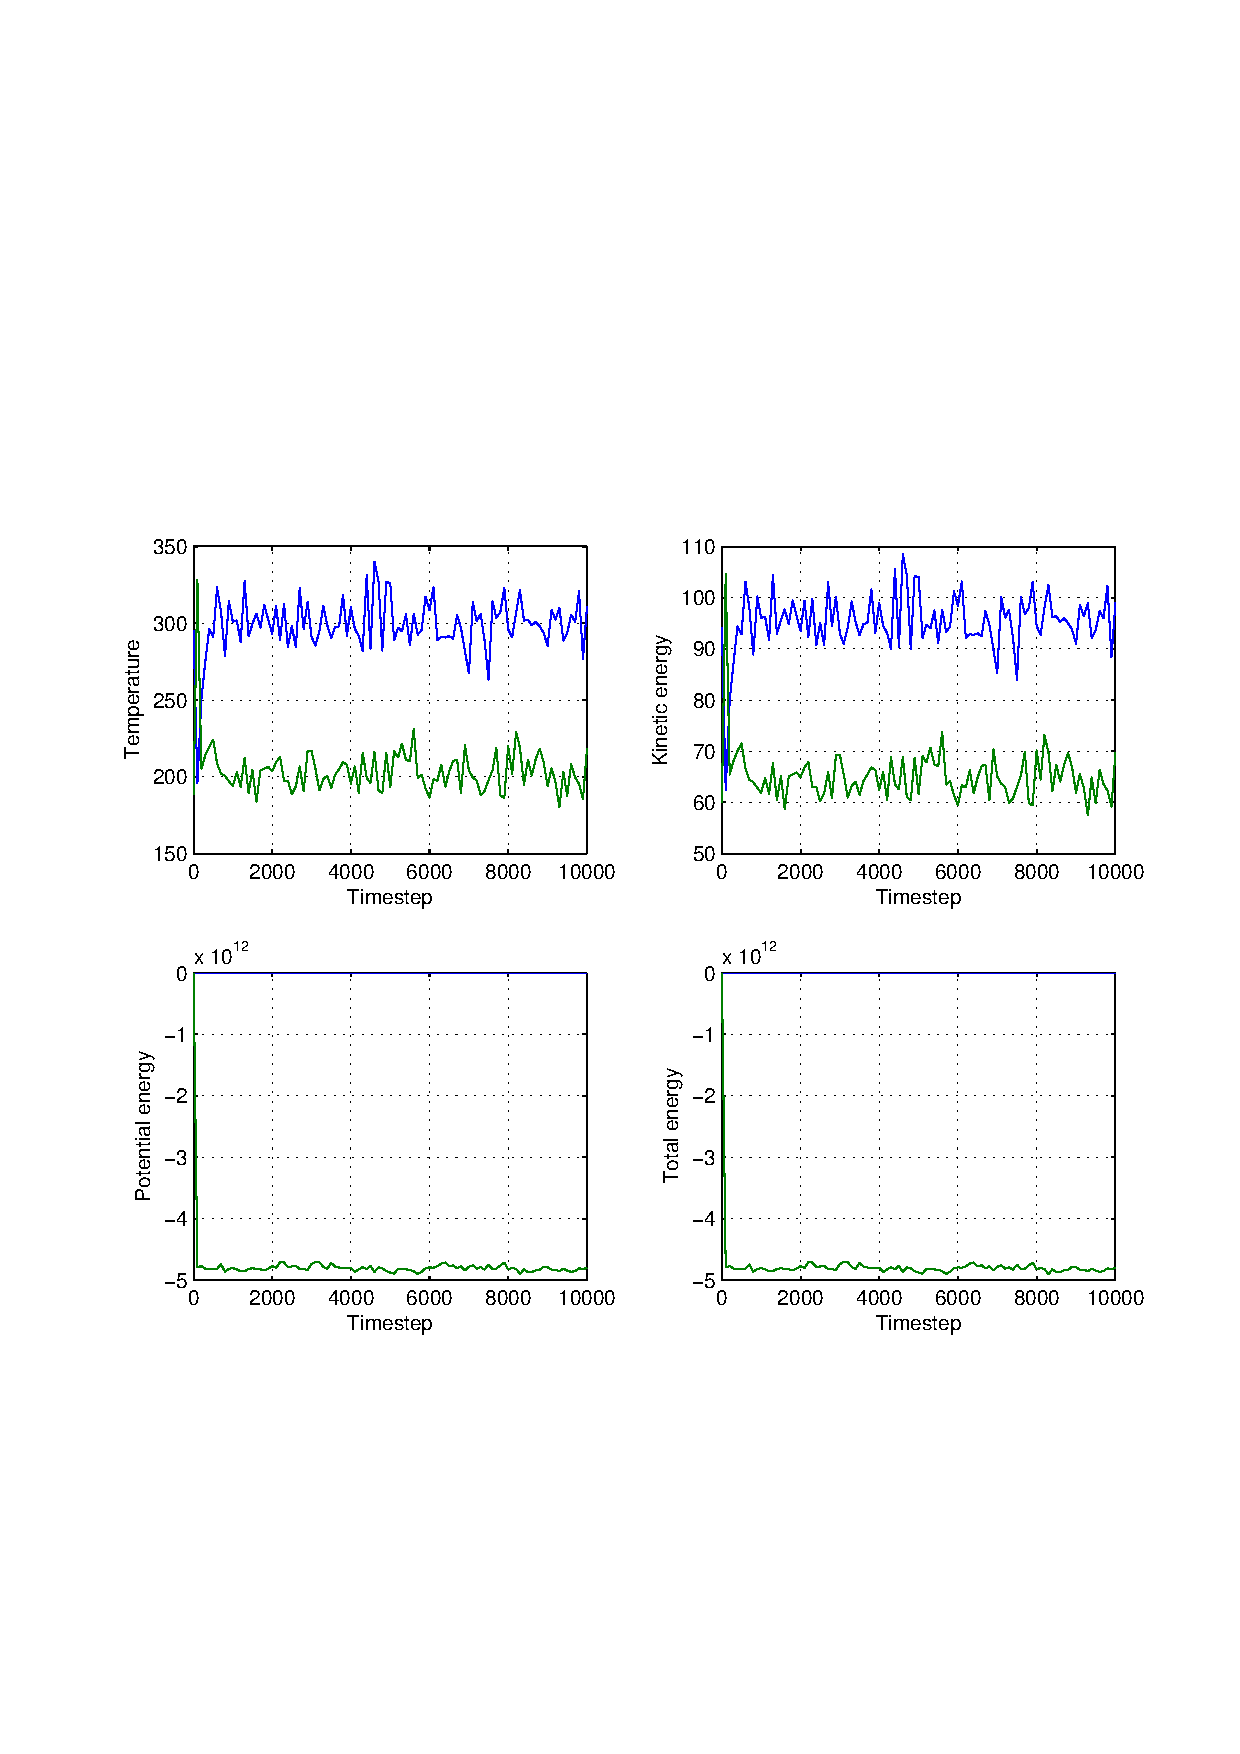
\includegraphics[totalheight=0.4\textheight]{partbf}
\caption{Comparision between LJ potential at 300K (Blue) and Buckingham Potential at 200K (Green)}
\label{fig:aNicePicture}
\end{figure}




\end{document}

